% Auto-generated by 04_additional_analysis.R — do not edit
% y > 0: Overreacts  |  y < 0: Underreacts
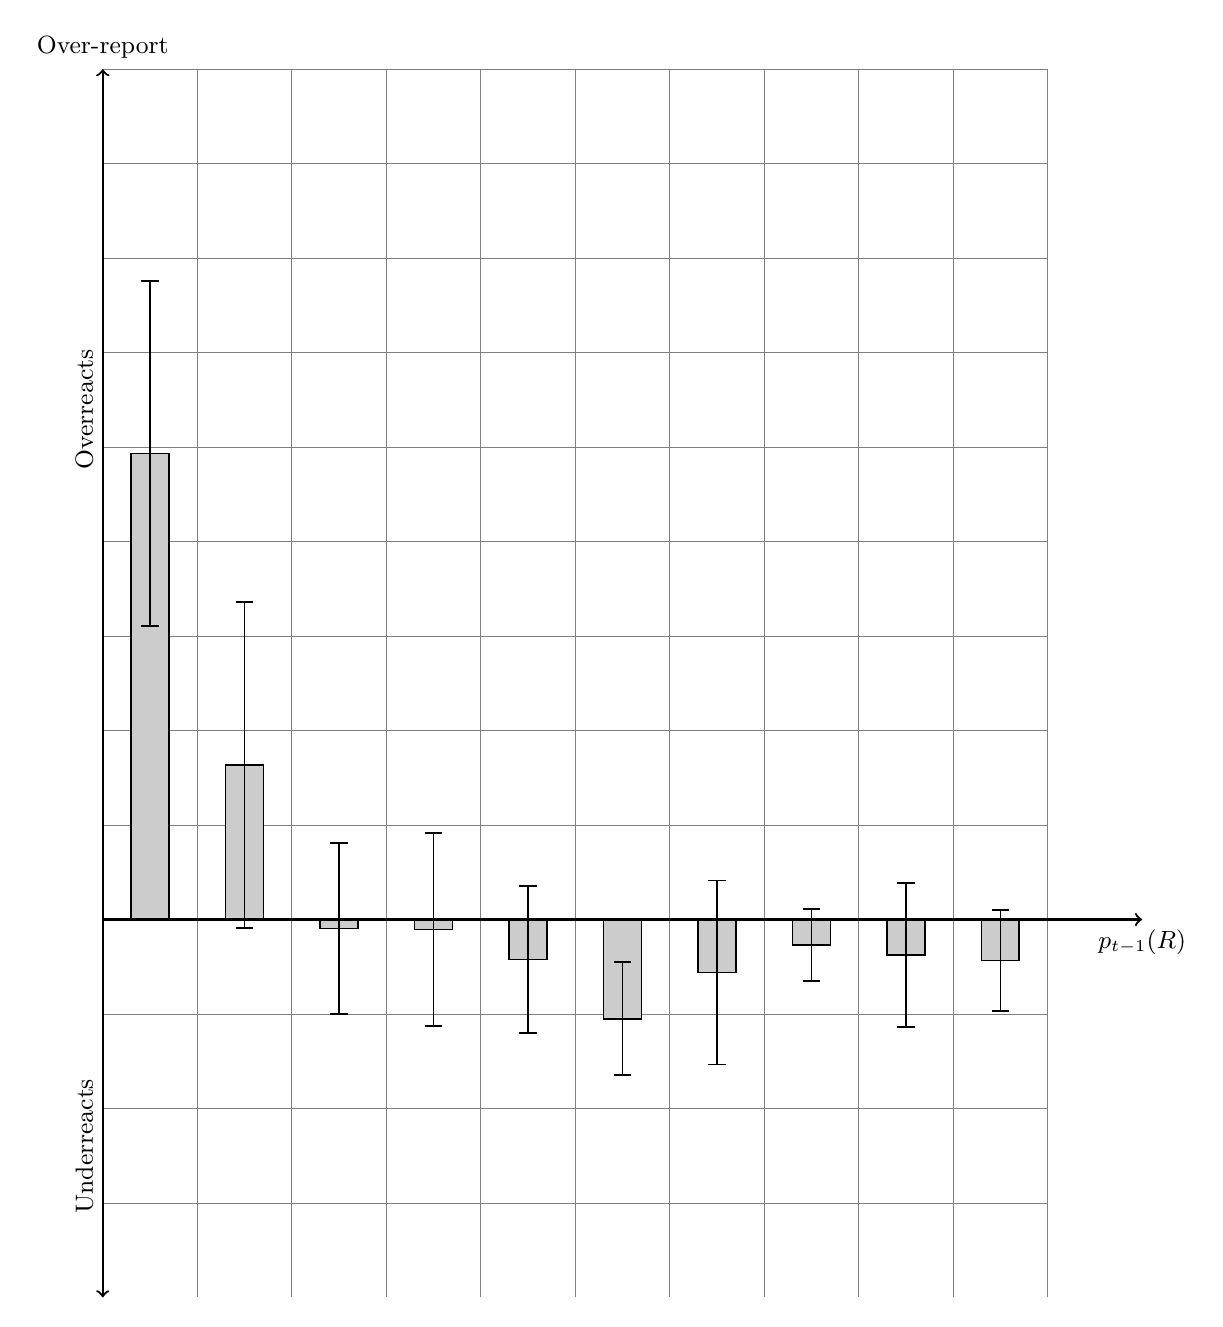
\begin{tikzpicture}[scale=12]
\draw[help lines,step=0.1] (0,-0.4) grid (1,0.9);
\filldraw[opaque,white!80!black] (0.03,0) rectangle (0.07,0.4931);
\draw[line width=0.6] (0.03,0) rectangle (0.07,0.4931);
\draw[line width=0.6,|-|] (0.05,0.3094) -- (0.05,0.6767);
\filldraw[opaque,white!80!black] (0.13,0) rectangle (0.17,0.1638);
\draw[line width=0.6] (0.13,0) rectangle (0.17,0.1638);
\draw[line width=0.6,|-|] (0.15,-0.0096) -- (0.15,0.3372);
\filldraw[opaque,white!80!black] (0.23,0) rectangle (0.27,-0.0095);
\draw[line width=0.6] (0.23,0) rectangle (0.27,-0.0095);
\draw[line width=0.6,|-|] (0.25,-0.1011) -- (0.25,0.0821);
\filldraw[opaque,white!80!black] (0.33,0) rectangle (0.37,-0.0105);
\draw[line width=0.6] (0.33,0) rectangle (0.37,-0.0105);
\draw[line width=0.6,|-|] (0.35,-0.1133) -- (0.35,0.0924);
\filldraw[opaque,white!80!black] (0.43,0) rectangle (0.47,-0.0423);
\draw[line width=0.6] (0.43,0) rectangle (0.47,-0.0423);
\draw[line width=0.6,|-|] (0.45,-0.1207) -- (0.45,0.0361);
\filldraw[opaque,white!80!black] (0.53,0) rectangle (0.57,-0.1051);
\draw[line width=0.6] (0.53,0) rectangle (0.57,-0.1051);
\draw[line width=0.6,|-|] (0.55,-0.1658) -- (0.55,-0.0444);
\filldraw[opaque,white!80!black] (0.63,0) rectangle (0.67,-0.0560);
\draw[line width=0.6] (0.63,0) rectangle (0.67,-0.0560);
\draw[line width=0.6,|-|] (0.65,-0.1542) -- (0.65,0.0423);
\filldraw[opaque,white!80!black] (0.73,0) rectangle (0.77,-0.0270);
\draw[line width=0.6] (0.73,0) rectangle (0.77,-0.0270);
\draw[line width=0.6,|-|] (0.75,-0.0661) -- (0.75,0.0122);
\filldraw[opaque,white!80!black] (0.83,0) rectangle (0.87,-0.0377);
\draw[line width=0.6] (0.83,0) rectangle (0.87,-0.0377);
\draw[line width=0.6,|-|] (0.85,-0.1145) -- (0.85,0.0392);
\filldraw[opaque,white!80!black] (0.93,0) rectangle (0.97,-0.0436);
\draw[line width=0.6] (0.93,0) rectangle (0.97,-0.0436);
\draw[line width=0.6,|-|] (0.95,-0.0979) -- (0.95,0.0107);
\draw[line width=0.8,->]  (0,0) -- (1.1,0) node[below] {\small{$p_{t-1}(R)$}};
\draw[line width=0.8,<->] (0,-0.4) -- (0,0.9) node[above] {\small{Over-report}};
\draw (0,0.54) node[above,rotate=90] {\small{Overreacts}};
\draw (0,-0.24) node[above,rotate=90] {\small{Underreacts}};
% ADD THEORY CURVE BELOW
\end{tikzpicture}
